\section{Theoretical Foundations}\label{sec:theory}
\subsection{Logical Systems and First-Order Logic}

\definition[Logical System]{
A \textbf{logical system} (or simply a \textbf{logic}) is a triple $\mathcal{S}:=\tuple{\mathcal{L},\mathcal{M},\vDash}$, where
\begin{itemize}
    \item $\mathcal{L}$ is a set of propositions
    \item $\mathcal{M}$ is a set of \textbf{models}, 
    \item $\vDash$ is a relation $\vDash \subseteq \mathcal{M} \times \mathcal{L}$ called the \textbf{satisfaction relation}. We read $\mathcal{M} \vDash A$ as $\mathcal{M}$ \textbf{satisfies} $A$ and correspondingly $\mathcal{M} \nvDash A$ as $\mathcal{M}$ \textbf{falsifies} $A$
\end{itemize}
}{logical_system}

\definition{
Let $\tuple{\mathcal{L},\mathcal{M},\vDash}$ be a logical system, $M \in \mathcal{M}$ a model and $A \in \mathcal{L}$ a proposition. Then we say that $A$ is
\begin{itemize}
\item \refterm{satisfied}{satisfied_ls} by $M$ iff $M \vDash A$
\item \refterm{satisfiable}{satisfiable_ls} iff $A$ is satisfied by some model
\item \refterm{unsatisfiable}{unsatisfiable_ls} iff $A$ is not satisfiable
\item \refterm{falsified}{falsified_ls} by $M$ iff $M \nvDash A$
\item \refterm{valid}{valid_ls} or \textbf{unfalsifiable} (write $\vDash A$) iff $A$ is satisfied by \textbf{every} model $M \in \mathcal{M}$
\item \refterm{invalid}{invalid_ls} or \textbf{falsifiable} (write $\nvDash A$) iff $A$ is not valid
\end{itemize}
}{}

\definition[Derivation Relation ($\vdash$)]{
Let $\mathcal{L}$ be a formal language.  
For any set of propositions $\mathcal{H} \subseteq \mathcal{L}$ (\textit{called the context or hypotheses}) and any proposition $A \in \mathcal{L}$, we write $\mathcal{H} \vdash A$ to say that $A$ is derivable from $\mathcal{H}$.  
We call a relation $\vdash \subseteq \powerset{\mathcal{L}} \times \mathcal{L}$ a \textbf{derivation relation} for $\mathcal{L}$, iff
\begin{itemize}
    \item $\mathcal{H} \vdash A$, if $A \in \mathcal{H}$ (proof reflexive),
    \item $\mathcal{H} \vdash A$ and $(\mathcal{H}' \cup \set{A}) \vdash B$ imply $(\mathcal{H} \cup \mathcal{H}') \vdash B$ (proof transitive),
    \item $\mathcal{H} \vdash A$ and $\mathcal{H} \subseteq \mathcal{H}'$ imply $\mathcal{H}' \vdash A$ (monotonic admits weakening).
\end{itemize}
}{derivation_relation_logic}

\definition[Inference Rules]{
Let $\mathcal{L}$ be a formal language, then an \textbf{inference rule} over $\mathcal{L}$ is decidable $n+1$-ary relation on $\mathcal{L}$. Inference rules are traditionally written as:
\[
\infer[\mathcal{N}]{C}{A_{1} \quad \dots \quad A_{n}}
\]

where $A_1, \cdots, A_n$ and $C$ are schemata for words in $\mathcal{L}$ and $\mathcal{N}$ is a name. The $A_i$ are called \textbf{assumptions} of $\mathcal{N}$, and $C$ is called its \textbf{conclusion}.


Any $n+1$-tuple $\infer[]{c}{a_{1} \quad \dots \quad a_{n}}$ in $\mathcal{N}$ is called an \textbf{application} of $\mathcal{N}$ and we say that we apply $\mathcal{N}$ to a set $M$ of words with $a_1, \cdots, a_n \in M$ to obtain $c$.
}{inference_rules_logic}

\definition[Axiom]{
An inference rule without assumptions is called an \textbf{axiom} (\texttt{Ax})
}{axiom_logic}

\definition[Calculus]{
A \textbf{calculus} (or \textbf{inference system}) is a formal language $\mathcal{L}$ equipped with a set $\mathcal{C}$ of inference rules over $\mathcal{L}$.
}{calculus_logic}


\definition[$\mathcal{C}$-derivation]{
Let $S := \tuple{\mathcal{L},\mathcal{M},\vDash}$ be a logical system, and $\mathcal{C}$ a calculus for $\mathcal{L}$, then a $\mathcal{C}$-derivation of a proposition $P \in \mathcal{L}$ from a set $\mathcal{H} \subseteq \mathcal{L}$ of hypotheses (write $\mathcal{H} \vdash_{\mathcal{C}}P$) is a sequence $A_1, \cdots, A_m$ of propositions where:
\begin{itemize}
\item $A_m = P$,
\item for all $1 \leq i \leq m$, either $A_i \in \mathcal{H}$, or,
\item there is an inference rule $\infer[\mathcal{N}]{A_i}{A_{l_1} \quad \dots \quad A_{l_k}}$ in $\mathcal{C}$ with $l_j < i$ for all $j \leq k$
\end{itemize}

We can also see a $\mathcal{C}$-derivation as a \textbf{derivation tree}, where $A_{l_j}$ are the children of the node $A_i$
}{c_derivation}

\definition[$\mathcal{C}$-refutation]{
Let $\mathcal{C}$ be a calculus, then a formula set $\Phi$ is called $\mathcal{C}$\textbf{-refutable} if there is a $\mathcal{C}$\textbf{-refutation}, i.e. a $\mathcal{C}$-derivation of a contradiction from $\Phi$. The act of finding a \textbf{refutation} for $\Phi$ is called \textbf{refuting} $\Phi$
}{c_refutation}

\definition[Soundness]{
Let $\mathcal{S}:=\tuple{\mathcal{L},\mathcal{M},\vDash}$ be a logical system and $\mathcal{H} \subseteq \mathcal{L}$ a set of hypotheses, then we call a calculus $\mathcal{C}$ over $\mathcal{L}$ \textbf{sound} (correct), iff $\mathcal{H} \sat A$ whenever $\mathcal{H} \vdash_{\mathcal{C}} A$
}{sound}

\definition[Completeness]{
Let $\mathcal{S}:=\tuple{\mathcal{L},\mathcal{M},\vDash}$ be a logical system and $\mathcal{H} \subseteq \mathcal{L}$ a set of hypotheses, then we call a calculus $\mathcal{C}$ over $\mathcal{L}$ \textbf{complete}, iff $\mathcal{H} \vdash_{\mathcal{C}} A$ whenever $\mathcal{H} \sat A$ 
}{complete}

\definition[Formal System]{
Let $\mathcal{S} := \langle \mathcal{L}, \mathcal{M}, \vDash \rangle$ be a logical system, and let $\mathcal{C}$ be a calculus over the language $\mathcal{L}$. Then the pair $\langle \mathcal{S}, \mathcal{C} \rangle$ is called a \textbf{formal system}.
}{formal_system}

\definition[Theorem Proving]{
Given a formal system $\tuple{\mathcal{S}, \mathcal{C}}$, where $\mathcal{C}$ is a calculus and $\mathcal{S} := \langle \mathcal{L}, \mathcal{M}, \vDash \rangle$ is a logical system, the task of \textbf{theorem proving} is the task of determining whether $\mathcal{H} \vdash_{\mathcal{C}} C$ for a \textbf{conjecture} $C \in \mathcal{L}$ and hypotheses $\mathcal{H} \subseteq \mathcal{L}$
}{theorem_proving}


\definition{
Prolog uses a simple calculus consisting of the following inference rules to build the knowledge base:
\begin{itemize}
    \item Modus Ponens (MP)
    \item Conjunction Introduction ($\land I$)
    \item Substitution (\texttt{Subst})
\end{itemize}

\[
    \infer[\text{MP}]
    {B}
    {A \Rightarrow B \quad A}
    \qquad
    \infer[\land I]
    {A \land B}
    {A \quad B} 
    \qquad
    \infer[\texttt{Subst}]
    {[B/X](A)}
    {A}
\]
}{}


\definition[Propositional Logic]{
Propositional Logic ($\text{PL}^0$) is a logical system $\tuple{\mathcal{L},\mathcal{M},\vDash}$ Where
\begin{itemize}
    \item the formal language $\mathcal{L}$ is defined as the well-formed formulae of propositional logic: $\text{wff}_0(\Sigma_{\text{PL}^0}, \mathcal{V}_{\text{PL}^0})$,
    \item the set $\mathcal{M}$ of models is given by the set $\mathcal{K}_0$ of total functions $\func{\varphi}{\mathcal{V}_0}{\mathcal{D}_0}$ (i.e., propositional variable assignments), 
    \item and $\varphi \vDash A$ iff $\mathcal{I}_{\varphi}(A) = T$ (a proposition is satisfiable by model $\varphi$ if the interpretation of it -under that $\varphi$- is true)
\end{itemize}
Hence, propositional logic is a logical system $\tuple{\text{wff}_0(\Sigma_{\text{PL}^0}, \mathcal{V}_{\text{PL}^0}),\mathcal{K}_0,\vDash}$
}{def:pl0_as_ls}

\definition[Formulae of $\text{PL}^0$]{
The formulae of $\text{PL}^0$ are made up from 
\begin{itemize}
    \item propositional variables $\mathcal{V}_{\text{PL}^0}$ (or just $\mathcal{V}_0$) : $\mathcal{V}_0 := \set{P,Q,R, \cdots}$ (countably infinite)
    \item propositional signature $\Sigma_{\text{PL}^0}$ (or just $\Sigma_0$): $\Sigma_0 := \set{\top,\bot,\neg, \lor, \land, \Rightarrow, \Leftrightarrow, \cdots}$ (called \textit{connectives})
\end{itemize}
We define the set $\text{wff}_0(\Sigma_{\text{PL}^0}, \mathcal{V}_{\text{PL}^0})$ of \textbf{well-formed propositional formulae (wffs)} as:
\begin{itemize}
    \item propositional variables
    \item logical constants $\top$ and $\bot$
    \item negations $\neg A$
    \item conjunctions $A \land B$
    \item disjunctions $A \lor B$
    \item implications $A \Rightarrow B$, and 
    \item equivalence (biimplications) $A \Leftrightarrow B$
\end{itemize}
where $A,B \in \text{wff}_0(\Sigma_{\text{PL}^0}, \mathcal{V}_{\text{PL}^0})$ themselves.
}{wff0_def}

\definition[$\text{PL}^1$]{
First-Order (Predicate) Logic $\text{PL}^1$ is a formal system that combines propositional logic ($\text{PL}^0$) with the ability to quantify over individuals
}{pl1}

\definition[First-Order Signature]{
A First-Order Signature is a tuple $\Sigma := \tuple{\Sigma_1, \Sigma_0}$ where $\Sigma_1 := \Sigma^f \cup \Sigma^p \cup \Sigma^{sk}$:
\begin{itemize}
\item $\Sigma^f := \bigcup_{k \in \mathbb{N}} \Sigma_k^f$ of \textbf{function constants} (or \textbf{terms}), where members of $\Sigma_k^f$ denote the $k$-ary functions on \textbf{individuals}
\item $\Sigma^p := \bigcup_{k \in \mathbb{N}} \Sigma_k^p$ of \textbf{predicate constants}, where members of $\Sigma_k^p$ denote $k$-ary relations among individuals
\item $\Sigma^{sk} := \bigcup_{k \in \mathbb{N}} \Sigma_k^{sk}$ of \textbf{Skolem constants} that act as witness constructors
\item All are pairwise disjoint, countable sets of symbols for each $k \in \mathbb{N}$.
\end{itemize}
We also assume a set of \textbf{individual variables} $V_{\iota} := \set{X,Y,Z,\cdots}$ which we can quantify over them.
}{fol_sig_pl1}

\definition[$\text{PL}^1$ Terms]{
The set $\text{wff}_{\iota}(\Sigma_1, V_{\iota})$ of \textbf{well-formed terms} over the signature $\Sigma_1$ and variables $V_{\iota}$ is defined by the following grammar:
\begin{align*}
f^k \quad &\in \quad \Sigma_k^f \cup \Sigma_k^{sk} \\
X \quad &\in \quad V_{\iota} \\ 
t \quad &::= \quad X \mid f^k(t_1, \cdots, t_k)
\end{align*}
}{terms_pl1}


\definition[$\text{PL}^1$ Propositions]{
The set $\text{wff}_{\circ}(\Sigma_1, V_{\iota})$ of \textbf{well-formed formulae} over the signature $\Sigma_1$ and variables $V_{\iota}$ is defined by the following grammar:
\begin{align*}
p^k \quad &\in \quad \Sigma_k^p \\
t_i \quad &\in \quad \text{wff}_{\iota}(\Sigma_1, V_{\iota}) \\ 
X \quad &\in \quad V_{\iota} \\ 
A \quad &::= \quad p^k(t_1, \cdots, t_k) \mid \top \mid \neg A \mid A \land A \mid \forall X.A
\end{align*}
}{formulae_pl1}

\definition[Free Variables]{
An occurrence of a variable $X$ is \textbf{free} in a formula $A$ if it is not within the scope of a binder. We define the set of free variables in $A$ ($\text{free}(A)$) recursively as follows:
\begin{itemize}
    \item \textbf{For Terms} ($t \in $ $\text{wff}_{\iota}(\Sigma_1, V_{\iota})$)
    \begin{itemize}
        \item $\text{free}(X) = \set{X}$
        \item $\text{free}(f^k(t_1, \cdots, t_k)) := \bigcup_{i=1}^{k} \text{free}(t_i)$
    \end{itemize}
    \item \textbf{For Formulae} ($A \in $ $\text{wff}_{\circ}(\Sigma_1, V_{\iota})$)
    \begin{itemize}
        \item $\text{free}(p^k(t_1, \cdots, t_k)) := \bigcup_{i=1}^{k} \text{free}(t_i)$
        \item $\text{free}(\top) := \emptyset$
        \item $\text{free}(\neg A) := \text{free}(A)$
        \item $\text{free}(A \land B) := \text{free}(A) \cup \text{free}(B)$
        \item $\text{free}(\forall X.A) := \text{free}(A) \setminus \set{X}$
    \end{itemize}
\end{itemize}
}{free_vars_pl1}

\definition[Bound Variables]{
An occurrence of a variable $X$ is \textbf{bound} if it occurs within the scope of a quantifier. We define the set of bound variables $\text{BVar}(A)$ as the set of all variables that are \textit{captured} by a binder:
\begin{itemize}
    \item \textbf{For Terms} ($t \in $ $\text{wff}_{\iota}(\Sigma_1, V_{\iota})$)
    \begin{itemize}
        \item $\text{BVar}(t) := \emptyset$ (\textit{variables in terms are always free until a formula provides a binder})
    \end{itemize}
    \item \textbf{For Formulae} ($A \in $ $\text{wff}_{\circ}(\Sigma_1, V_{\iota})$)
    \begin{itemize}
        \item $\text{BVar}(p^k(t_1, \cdots, t_k)) := \emptyset$
        \item $\text{BVar}(\neg A) := \text{BVar}(A)$
        \item $\text{BVar}(A \land B) := \text{BVar}(A) \cup \text{BVar}(B)$
        \item $\text{BVar}(\forall X.A) := \text{BVar}(A) \cup \set{X}$
    \end{itemize}
\end{itemize}
}{bound_vars_pl1}

\definition[Ground Formulae]{
A $\text{PL}^1$ formula $A$ is called \textbf{ground/closed} iff free$(A) := \emptyset$. A closed formula is called a sentence. We denote the set of all \textbf{ground} terms with $\text{cwff}_{\iota}(\Sigma_1, V_{\iota})$ and the set of all sentences with $\text{cwff}_{\circ}(\Sigma_1, V_{\iota})$
}{ground_pl1}

\definition[Alphabetical Variants]{
Bound variables can be \textbf{renamed}; specifically, if $\forall X.B$ is a sub-formula of $A$, let $A'$ be the result of replacing $\forall X.B$ in $A$ with $\forall Y.B'$, where $B'$ is obtained from $B$ by replacing all occurrences of $X \in \text{free}(B)$ with a new variable $Y$ that does not occur in $A$. We call $A'$ an \textbf{alphabetical variant} of $A$ (and vice versa).
}{alphabetical_variants}

\definition[Expression Language]{
Let signature $\Sigma$ and variables $\mathcal{V}$ be disjoint sets and $G$ a grammar whose vocabulary is $\Sigma \cup \mathcal{V}$, then we call $\tuple{\Sigma, \mathcal{V}, G}$ an \textbf{expression language}, and denote the language of $G$ with $\text{wfe}(\Sigma, \mathcal{V})$: the set of \textbf{well-formed expressions}.
}{expression_language}

\commandnote{
For $\text{PL}^1$, we have:
\[
\text{wfe}(\Sigma_1, \mathcal{V}_{\iota}) := \text{wff}_{\circ}(\Sigma_1, V_{\iota}) \cup \text{wff}_{\iota}(\Sigma_1, V_{\iota})
\]
}

\subsection{Substitutions and Unification}
\definition[Support]{
Let $f: A \to B$ be a function. The \textbf{support} of $f$, denoted by $\text{supp}(f)$, is the set of all elements in the domain $A$ for which the function does not return a "default" or "identity" value. 
}{support_function}

\begin{example}[Default is Zero]{}
Let $f: \mathbb{Z} \to \mathbb{Z}$ be a function that assigns almost every integer to $0$, except:
\[
f(2) = 5, \quad f(7) = -3, \quad \text{and} \quad f(x) = 0 \text{ for all other } x \in \mathbb{Z}.
\]
The ``default'' value is $0$. Therefore, the support consists only of the points that deviate from $0$:
\[
\text{supp}(f) = \{2, \, 7\}
\]   
\end{example}

\begin{example}[Default is Identity]{}
Consider a variable mapping $\sigma$ over an infinite set of variables $\mathcal{V} = \{X, Y, Z, W, \dots\}$ where the default behavior is to leave a variable unchanged ($\sigma(V) = V$).

If $\sigma$ only modifies two variables:
\[
\sigma(X) = a, \quad \sigma(Y) = g(Z), \quad \text{and} \quad \sigma(V) = V \text{ for all other } V \in \mathcal{V},
\]
then the support of $\sigma$ is precisely the finite set of variables whose values actually change:
\[
\text{supp}(\sigma) = \{X, \, Y\}
\]   
\end{example}


\definition[Substitution]{
Let $\text{wfe}(\Sigma, \mathcal{V})$ be an expression language, then we call $\func{\sigma}{\mathcal{V}}{\text{wfe}(\Sigma, \mathcal{V})}$ a \textbf{substitution} iff the support $\text{supp}(\sigma) := \set{X \mid (X,A) \in \sigma \land X \neq A}$ of $\sigma$ is finite. We denote the \textbf{empty substitution} with $\epsilon$.
}{substitution}

\definition{
We can \textbf{discharge} a variable $X$ from a substitution $\sigma$ by setting $\sigma_{-X} := \sigma , [X/X]$
}{discharge_substitution}

\definition[Introduced Variables]{
Let $\sigma$ be a substitution. The set of variables \textbf{introduced} by $\sigma$, denoted by $\text{intro}(\sigma)$, is the set of all free variables occurring in the replacement terms:
\[
\text{intro}(\sigma) := \bigcup_{X \in \text{supp}(\sigma)} \text{free}(\sigma(X))
\]
}{intro_substitution}

\begin{example}{}
consider the formula $A := \forall X. p(X,Y)$ and the substitution $\sigma := \set{[Z / Y]}$:
\begin{itemize}
    \item $\text{supp}(\sigma) = \set{Y}$
    \item $\text{free}(\sigma(Y)) = \text{free}(Z) = \set{Z}$
    \item $\text{intro}(\sigma) = \text{free}(\sigma(Y)) = \set{Z}$
\end{itemize}
\end{example}

\definition[Substitution Application]{
We define substitution application by:
\begin{itemize}
    \item $\sigma(c) = c$ for $c \in \Sigma$
    \item $\sigma(X) = A$ iff $X \in \mathcal{V}$ and $(X,A) \in \sigma$
    \item $\sigma(f(A_1, \cdots, A_n)) = f(\sigma(A_1), \cdots, \sigma(A_n))$
    \item $\sigma(\forall X.A) = \forall X.\sigma_{-X}(A)$
\end{itemize}
}{substitution_application}

\begin{example}{}
consider the formula $g(x,y, h(z))$, and we want to apply the substitution $\sigma := \set{x \mapsto a, y \mapsto f(b), z \mapsto a}$ we get the formula $g(a, f(b), h(a))$    
\end{example}

\notationbox{
Usually we use another notation for writing the substitution $\sigma := \set{x \mapsto a, y \mapsto f(b), z \mapsto a}$ which is $[a/x], [f(b) / y], [a / z]$ where $[A / X]$ (read as \textit{A for X} i.e. substitute $X$ with $A$) $\equiv X \mapsto A \equiv (X,A) \in \sigma$ 
}

\definition{
Let $\sigma$ be a substitution, $A$ a formula, and $A'$ an alphabetical variant of $A$, such that $\text{intro}(\sigma) \cap \text{BVar}(A') = \emptyset$. Then we define \textbf{capture-avoiding substitution application} via $\sigma(A) := \sigma(A')$
}{subst_app_avoid_capture}

\commandnote{
We said $\sigma(\forall X.A) = \forall X.\sigma_{-X}(A)$ but this can lead to \refterm{variable capture}{variable_capture}, i.e. $[f(X) / Y](\forall X.p(X,Y))$ would evaluate to $\forall X.p(X,f(X))$ where the second occurrence of $X$ is now bound whereas it was free before.

The solution for this is to rename the bound variable $X$ in $\forall X.p(X,Y)$ before applying the substitution and there where we need capture-avoiding substitution application 
}

\begin{example}{}
we want to apply $\sigma := \set{[f(X) / Y]}$ to the formula $A = \forall X. p(X,Y)$
\begin{itemize}
    \item $\text{intro}(\sigma) \cap \text{BVar}(A) = \set{X} \cap \set{X} = \set{X}$ 
    \item Hence, we need to find an alphabetical variant $A'$ for $A$, say $A' = \forall Z. p(Z,Y)$
    \item Now $\text{intro}(\sigma) \cap \text{BVar}(A') = \set{X} \cap \set{Z} = \emptyset$
    \item Hence, we define $\sigma(A) = \sigma(A')$
    \item $\sigma(A') = \sigma(\forall Z. p(Z,Y)) = \forall Z. \sigma_{-Z} (p(Z,Y))$
    \item $[f(X) / Y](p(Z,Y)) = p(Z,f(X))$
    \item $\sigma(A) = \sigma(A') = \forall Z.p(Z,f(X))$
\end{itemize}
\end{example}

\definition[Unification]{
For given terms $A_1, A_2$, \textbf{unification} is the problem of finding a substitution $\sigma$ (called \textbf{unifier}), such that $\sigma(A_1)=\sigma(A_2)$
}{}


\definition[Unification Problem]{
We call a formula $A^1 =^? B^1 \land \cdots \land A^n =^? B^n$ a \textbf{unification problem} iff $A^i, B^i \in$ $\text{wff}_{\iota}(\Sigma_1, V_{\iota})$
}{unification_problem}

\definition{
A substitution is called a \textbf{unifier} for a unification problem $\mathcal{E}$ (and thus $\mathcal{E}$ is \textbf{unifiable}), iff it is a (simultaneous) unifier for all pairs in $\mathcal{E}$ 
}{unifier_unifiable}

\definition{
The solution for a unification problem $U(A_1, A_2)$ is the set of unifiers $\set{\sigma \mid \sigma(A_1) = \sigma(A_2)}$. For example, let $\mathcal{E} := f(X) =^? f(g(Y))$, solutions are, e.g.
\begin{itemize}
\item $[g(a)/X], [a/Y]$
\item $[g(g(a))/X], [g(a)/Y]$
\item $[g(Z)/X], [Z/Y]$
\item $[g(Y)/X]$
\end{itemize}
}{}

\definition{
Let $\sigma$ and $\theta$ be substitutions and $W \subseteq \mathcal{V}_{\iota}$, we say that a substitution $\sigma$ is \textbf{more general} than $\theta$ on $W$ (write as $\sigma \leq \theta[W]$), iff there is a substitution $\rho$, such that $\theta = \rho \circ \sigma[W]$, where $\sigma = \rho[W]$, iff $\sigma(X) = \rho(X)$ for all $X \in W$
}{more_general_subst}

\commandnote{
\begin{itemize}
    \item The substitution $\sigma = [g(Z)/X, Z/Y]$ is more general than $\theta = [g(a)/X, a/Y]$ because there exists $\rho = [a/Z]$ such that:
    \[ \theta = \rho \circ \sigma \]
    This identity $\theta = \rho \circ \sigma$ is verified by applying the composition to the variables in the domain:
    \begin{itemize}
        \item $(\rho \circ \sigma)(X) = \rho(\sigma(X)) = \rho(g(Z)) = g(a)$
        \item $(\rho \circ \sigma)(Y) = \rho(\sigma(Y)) = \rho(Z) = a$
    \end{itemize}
    Since the mapping for each variable matches $\theta$, we confirm that $\theta$ is a specialization of $\sigma$ via $\rho$.

    \item Likewise, $\sigma$ is more general than $\theta' = [g(g(a))/X, g(a)/Y]$ via $\rho' = [g(a)/Z]$, since:
    \[ \theta' = \rho' \circ \sigma \]
    where $(\rho' \circ \sigma)(X) = g(g(a))$ and $(\rho' \circ \sigma)(Y) = g(a)$.
\end{itemize}
}

\definition[MGU]{
$\sigma$ is called a \textbf{most general unifier (mgu)} of $A_1,A_2$, iff it is minimal in $U(A_1, A_2)$ \textbf{with respect to} the more general ordering ($\leq$) restricted to the variables occurring in the problem: $W = \text{free}(A_1) \cup \text{free}(A_2)$.
}{}

\definition{
We call a pair $A =^? B$ \textbf{solved} in a unification problem $\mathcal{E}$, iff $A$ is a variable $X$, $\mathcal{E} = X =^? A \land \mathcal{E'}$, and $X \notin (\text{free}(A) \cup \text{free}(\mathcal{E'}))$. We call a unification problem $\mathcal{E}$ a \textbf{solved form}, iff all its pairs are \textbf{solved}.
}{solved_unif_prob}

\Lemma{
Solved forms are of the form $X^1 =^? B^1 \land \cdots \land X^n =^? B^n$ where $X^i$ are distinct and $X^i \notin \text{free}(B^j)$
}{lemm:solved_forms}

\definition[$\mathcal{E}_{\sigma}$]{
Any substitution $\sigma = [B^1/X^1], \cdots , [B^n / X^n]$ induces a \textbf{solved unification problem} 
\[
\mathcal{E}_{\sigma} := (X^1 =^? B^1 \land \cdots \land X^n =^? B^n)
\]
}{solved_unification_problem}

\Lemma{
If $\mathcal{E} = X^1 =^? B^1 \land \cdots \land X^n =^? B^n$ is a solved form, then $\mathcal{E}$ has the unique MGU $\sigma_{\epsilon} := [B^1 / X^1], \cdots , [B^n / X^n]$.
}{}

\definition[$\mathcal{U}$]{
A unification engine $\mathcal{U}$ uses the following inference rules:
\begin{tcolorbox}[colback=white, colframe=black, sharp corners, boxrule=0.5pt]
    \begin{multicols}{2}
        \noindent
        \begin{minipage}{\linewidth}
            \[
            \infer[\mathcal{U}_{dec}]
            {\mathcal{E} \land A^1 =^? B^1 \land \cdots \land A^n =^? B^n}
            {\mathcal{E} \land f(A^1,\cdots,A^n) =^? f(B^1,\cdots,B^n)}
            \]
        \end{minipage}
    
        \noindent
        \begin{minipage}{\linewidth}
            \vspace{0.1cm}
            \[
            \infer[\mathcal{U}_{triv}]
            {\mathcal{E}}
            {\mathcal{E} \land A =^? A}
            \]
        \end{minipage}
    \end{multicols}

    \begin{multicols}{2}
        \noindent
        \begin{minipage}{\linewidth}
            \[
                \infer[\mathcal{U}_{elim}]
                {[A/X](\mathcal{E} \land X =^? A)}
                {\mathcal{E} \land X =^? A \quad X \notin free(A) \quad X \in free(\mathcal{E})}
            \]
        \end{minipage}

        \noindent
        \begin{minipage}{\linewidth}
            \vspace{0.4cm}
            \[
                \infer[\mathcal{U} \bot]
                {\bot}
                {\mathcal{E} \land f(X^1,\cdots,X^n) =^? g(Y^1,\cdots,Y^n)}
            \]
        \end{minipage}
    \end{multicols}
\end{tcolorbox}
}{}

\begin{example}[Unification]{}
Let $\mathcal{E} := f(g(X, X), h(a)) =^? f(g(a, Z), h(Z))$:

\begin{figure}[H]
    \centering
    \begin{tcolorbox}[colback=white, colframe=black, sharp corners, boxrule=0.5pt]
        \centering
        \vspace{0.3cm}
        \[
        \infer[\mathcal{U}_{triv}]
        {X =^? a \land Z =^? a}
        {
            \infer[\mathcal{U}_{elim}]
            {X =^? a \land Z =^? a \land a =^? a}
            {
                \infer[\mathcal{U}_{elim}]
                {X =^? a \land a =^? Z \land a =^? Z}
                {
                    \infer[\mathcal{U}_{dec}]
                    {X =^? a \land X =^? Z \land a =^? Z}
                    {
                        \infer[\mathcal{U}_{dec}]
                        {X =^? a \land X =^? Z \land h(a) =^? h(Z)}
                        {
                            \infer[\mathcal{U}_{dec}]
                            {g(X, X) =^? g(a, Z) \land h(a) =^? h(Z)}
                            {f(g(X, X), h(a)) =^? f(g(a, Z), h(Z))}
                        }
                    }
                }
            }
        }
        \]
        \vspace{0.1cm}
        The final $\mathcal{E}$ is in solved form since all the pairs are solved. Hence $\mathcal{E}$ has the unique MGU $\sigma_{\epsilon} := [a / X], [a / Z]$. 
    \end{tcolorbox}
\end{figure}
\end{example}

\begin{example}[Unification]{}
Let $\mathcal{E} := S_1(g(f(x), g(x, y)), y) =^? S_1(g(z, v), f(w))$

\begin{figure}[H]
    \centering
    \begin{tcolorbox}[colback=white, colframe=black, sharp corners, boxrule=0.5pt]
        \centering
        \vspace{0.3cm}
        \[
        \infer[\mathcal{U}_{elim}]
        {z =^? f(x) \land v =^? g(x, f(w)) \land y =^? f(w)}
        {
            \infer[\mathcal{U}_{elim}]
            {z =^? f(x) \land v =^? g(x, y) \land y =^? f(w)}
            {
                \infer[\mathcal{U}_{dec}]
                {z =^? f(x) \land v =^? g(x, y) \land y =^? f(w)}
                {
                    \infer[\mathcal{U}_{dec}]
                    {g(f(x), g(x, y)) =^? g(z, v) \land y =^? f(w)}
                    {S_1(g(f(x), g(x, y)), y) =^? S_1(g(z, v), f(w))}
                }
            }
        }
        \]
        \vspace{0.4cm}
        \flushleft
        The final equation $z =^? f(x) \land v =^? g(x, f(w)) \land y =^? f(w)$ is in solved form. \\
        The MGU is $\{z \to f(x), v \to g(x, f(w)), y \to f(w)\}$.
    \end{tcolorbox}
\end{figure}
\end{example}

\begin{example}[Unification Failure]{}
Let $\mathcal{E}:=S_2(g(f(x), g(x, u)), f(y), z) =^? S_2(g(g(g(u, v), f(w)), f(c)), f(g(u, v)), f(c))$

\begin{figure}[H]
    \centering
    \begin{tcolorbox}[colback=white, colframe=black, sharp corners, boxrule=0.5pt]
        \centering
        \[
        \infer[\mathcal{U} \bot]
        {\bot}
        {
            \infer[\mathcal{U}_{dec}]
            {f(x) =^? g(g(u, v), f(w)) \land g(x, u) =^? f(c) \land f(y) =^? f(g(u, v)) \land z =^? f(c)}
            {
                \infer[\mathcal{U}_{dec}]
                {g(f(x), g(x, u)) =^? g(g(g(u, v), f(w)), f(c)) \land f(y) =^? f(g(u, v)) \land z =^? f(c)}
                {S_2(g(f(x), g(x, u)), f(y), z) =^? S_2(g(g(g(u, v), f(w)), f(c)), f(g(u, v)), f(c))}
            }
        }
        \]
    \end{tcolorbox}
\end{figure}
\end{example}

\subsection{The Resolution Calculus}
\definition[Test Calculus]{
For a given conjecture $A$ and hypotheses $\mathcal{H}$, a \textbf{test calculus} $\mathcal{T}$ tries to derive a refutation $\mathcal{H}, \neg A \vdash_{\mathcal{T}} \bot$ instead of $\mathcal{H} \vdash A$, where $\neg A$ is unsatisfiable iff $A$ is valid and $\bot$ an unsatisfiable proposition.
}{test_calculus}

\definition{
A formula is called \textbf{atomic} (or an \textbf{atom}) if it does not contain logical constants, otherwise, \textbf{complex}
}{atomic_formula}

\definition[Labeled Formula]{
Let $\mathcal{S} := \langle \mathcal{L}, \mathcal{M}, \vDash \rangle$ be a logical system, $A \in \mathcal{L}$ a formula, $L$ a \textbf{label set}, and $\alpha \in L$ a \textbf{label}, then we call a pair $\tuple{A, \alpha}$ a \textbf{labeled formula} and write it as $A^{\alpha}$. For a set $\Phi$ of propositions we use $\Phi^{\alpha} := \set{A^{\alpha} \mid A \in \Phi}$
}{labeled_formula}

\commandnote{
If the label set is $\mathcal{D}_0 := \set{T,F}$, we call a labeled formula $A^T$ \textbf{positive} and $A^F$ \textbf{negative}
}

\commandnote{
Let $\mathcal{S} := \langle \mathcal{L}, \mathcal{M}, \vDash \rangle$ be a logical system, and $A^{\alpha}$ a labeled formula. Then we say that $M \in \mathcal{M}$ \textbf{satisfies} $A^{\alpha}$ (write $M \vDash A^{\alpha}$), iff $\alpha = T$ and $M \vDash A$ or $\alpha = F$ and $M \nvDash A$
}

\definition[Literal]{
Let $\mathcal{S} := \langle \mathcal{L}, \mathcal{M}, \vDash \rangle$ be a logical system, $A \in \mathcal{L}$ is an atomic formula, and $\alpha \in \set{T,F}$, then we call the labeled formula $A^{\alpha}$ a \textbf{literal}.
}{literal}

\definition[Opposite Literal]{
For a literal $A^{\alpha}$, we call the literal $A^{\beta}$ with $\alpha \neq \beta$ the opposite literal.
}{opposite_literal}

\definition[CNF]{
A formula is in \textbf{conjunctive normal form (CNF)} if it is $\top$ or a conjunction of disjunctions of literals, i.e. if it is of the form:
\[
\bigwedge_{i=1}^{n} \bigvee_{j=1}^{m_i} l_{ij} := 
\underbrace{
    \overbrace{( l_{1,1} \lor \dots \lor l_{1,m_1} )}^{\text{Clause } i=1 \text{ has } m_1 \text{ literals}}
    \land
    \overbrace{( l_{2,1} \lor \dots \lor l_{2,m_2} )}^{\text{Clause } i=2 \text{ has } m_2 \text{ literals}}
    \land \dots \land
    \overbrace{( l_{n,1} \lor \dots \lor l_{n,m_n} )}^{\text{Clause } i=n \text{ has } m_n \text{ literals}}
}_{\text{There are } n \text{ total clauses}}
\]
}{cnf}

\definition{
The \defemph{resolution calculus} (or simply \defemph{resolution}) is a test calculus consisting of the inference rules shown in \Figref{fig:r0_r1}
}{}

\begin{figure}[H]
    \centering
    \begin{tcolorbox}[colback=white, colframe=black, sharp corners, boxrule=0.5pt]
        \noindent
        \begin{minipage}{\linewidth}
            \[
            \infer[\mathcal{R}_0]
            {A \lor B}
            {P^T \lor A \qquad \qquad P^F \lor B}
            \]
        \end{minipage}
        \begin{multicols}{2}
            \noindent
            \begin{minipage}{\linewidth}
                \[
                    \infer[\mathcal{R}_1]
                    {(\sigma(C)) \lor (\sigma(D))}
                    {A^T \lor C \quad B^F \lor D \quad \sigma = \text{MGU}(A,B)}
                \]
            \end{minipage}

            \noindent
            \begin{minipage}{\linewidth}
                \[
                    \infer[\mathcal{R}_1]
                    {(\sigma(A)) \lor (\sigma(C))}
                    {A^{\alpha} \lor B^{\beta} \lor C \quad \sigma = \text{MGU}(A,B)}
                \]
            \end{minipage}
        \end{multicols}
    \end{tcolorbox}
    \caption{Resolution Calculus}
    \label{fig:r0_r1}
\end{figure}


\redbox{Resolution is the main machinery behind the Prolog inference engine}

\definition[Clause]{
A \textbf{clause} is a disjunction $l_1^{\alpha_1} \lor \cdots \lor l_n^{\alpha_n}$ of literals. We use $\square$ for the \textit{"empty"} disjunction (no disjuncts) and call it the \textbf{empty clause}. A clause with exactly one literal is called a \textbf{unit clause}.
}{clause_resolution}

\definition[Clause Set]{
We often write a \textbf{clause set} $\set{C_1, \cdots, C_n}$ as $C_1 ; \cdots ; C_n$, and write $S ; T$ for the union of the clause sets $S$ and $T$, and $S ; C$ for the extension of $S$ by a clause $C$.
}{clause_set}

\definition[Resolution Refutation]{
Let $S$ be a clause set, then we call an $\mathcal{R}$-derivation of the empty clause $\square$ from $S$ \textbf{$\mathcal{R}$-refutation} and write $\mathcal{D}: S \vdash_{\mathcal{R}} \square$.
}{resolution_refutation}

\begin{example}[Resolution Proof]{}
We want to prove the following propositional formula using resolution:
\[
(p \Rightarrow q \Rightarrow r) \Rightarrow (p \Rightarrow q) \Rightarrow p \Rightarrow r
\]

We negate it and try to derive the empty clause (refutation). After negating it and transforming it to CNF (since resolution works only on CNF), we get the following clause set:
\[
\Phi := \set{p^F \lor q^F \lor r^T , p^F \lor q^T , p^T , r^F}
\]

We start resolving:
\begin{table}[H]
\begin{tabular}{|l|l|l|} \hline
1 & $p^F \lor q^F \lor r^T$ & initial \\ \hline   
2 & $p^F \lor q^T$ & initial \\ \hline   
3 & $p^T$ & initial \\ \hline   
4 & $r^F$ & initial \\ \hline   
5 & $p^F \lor q^F$ & resolve 1.3 with 4.1 \\ \hline  
6 & $q^F$ & resolve 3.1 with 5.1 \\ \hline   
7 & $p^F$ & resolve 2.2 with 6.1 \\ \hline 
8 & $\square$ & resolve 3.1 with 7.1 \\ \hline   
\end{tabular}
\end{table}
\end{example}

\commandnote{
A resolution proof can be represented in a proof tree as shown in \Figref{fig:r0_proof_tree}
}

\begin{figure}[H]
\centering
\begin{tcolorbox}[colback=white, colframe=black, sharp corners, boxrule=0.5pt]
\centering
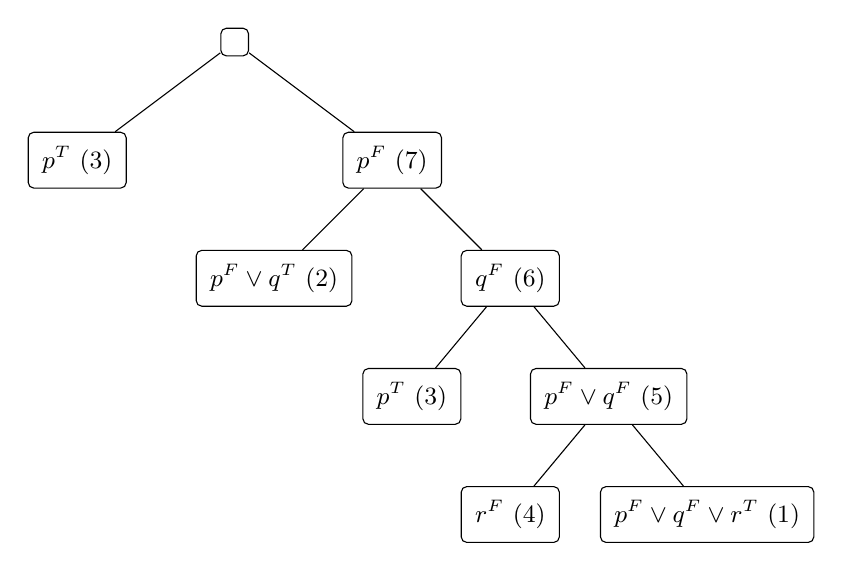
\begin{tikzpicture}[
  level distance=1.5cm,
  level 1/.style={sibling distance=4cm},
  level 2/.style={sibling distance=3cm},
  level 3/.style={sibling distance=2.5cm},
  edge from parent/.style={draw, thin},
  every node/.style={
    draw, 
    rectangle, 
    rounded corners=2pt, 
    inner sep=5pt, 
    font=\small
  }
]  
\node {$\square$}
  child {node {$p^T$ (3)}}
  child {node {$p^F$ (7)}
    child {node {$p^F \lor q^T$ (2)}}
    child {node {$q^F$ (6)}
      child {node {$p^T$ (3)}}
      child {node {$p^F \lor q^F$ (5)}
        child {node {$r^F$ (4)}}
        child {node {$p^F \lor q^F \lor r^T$ (1)}}
      }
    }
  };

\end{tikzpicture}    
\end{tcolorbox}
\caption{Resolution Proof Tree}
\label{fig:r0_proof_tree}
\end{figure}

\begin{example}[Resolution Given a Knowledge Base]{}
Consider we have a knowledge base $\text{KB} := \set{A \Rightarrow B \lor C , A, \neg B}$, we want to check if $\text{KB} \vDash C$. $\text{KB} \vDash C$ iff $\text{KB} \cup \set{\neg C}$ is unsatisfiable.

First we need to compute $\text{CNF} (A \Rightarrow B \lor C)$
\begin{itemize}
    \item $\text{CNF} (A \Rightarrow B \lor C) = \neg A \lor B \lor C$
\end{itemize}
$\text{KB} \cup \set{\neg C} := \set{\neg A \lor B \lor C, A, \neg B, \neg C} := \set{A^F \lor B^T \lor C^T, A^T, B^F, C^F}$

\begin{figure}[H]
\begin{tcolorbox}[colback=white, colframe=black, sharp corners, boxrule=0.5pt]
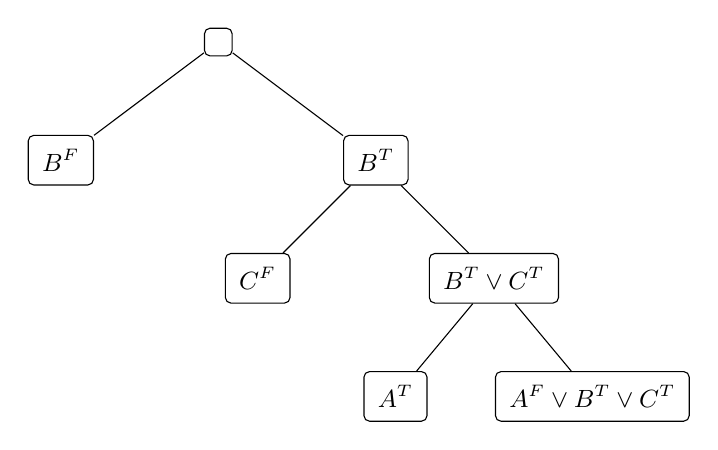
\begin{tikzpicture}[
  level distance=1.5cm,
  level 1/.style={sibling distance=4cm},
  level 2/.style={sibling distance=3cm},
  level 3/.style={sibling distance=2.5cm},
  edge from parent/.style={draw, thin},
  every node/.style={
    draw, 
    rectangle, 
    rounded corners=2pt, 
    inner sep=5pt, 
    font=\small
  }
]  
\node {$\square$}
  child {node {$B^F$}}
  child {node {$B^T$}
    child {node {$C^F$}}
    child {node {$B^T \lor C^T$}
      child {node {$A^T$}}
      child {node {$A^F \lor B^T \lor C^T$}
      }
    }
  };

\end{tikzpicture}  
\hfill
Since $\text{KB} \cup \set{\neg C}$ is unsatisfiable, $\text{KB} \vDash C$
\end{tcolorbox}
\end{figure}
\end{example}



\definition[Refutational Completeness]{
A test calculus $\mathcal{C}$ is called \textbf{refutationally complete} iff for every unsatisfiable clause set $\Phi$, there exists a refutation deriving the empty clause:
\[
\Phi \text{ is unsatisfiable} \iff \Phi \vdash_{\mathcal{C}} \square
\]
}{refutational_completeness}

\titledbox{Deductive vs. Refutational Completeness}{
Resolution is \textbf{not} deductively complete: from the clause set $\{p\}$, resolution cannot directly derive the valid consequence $p \lor q$. However, resolution is \textbf{sound and refutationally complete}: if we add the negation $\neg(p \lor q) \equiv p^F \land q^F$ to $\{p^T\}$, resolution is guaranteed to derive the contradiction $\square$.
}

\subsection{Horn Logic and SLD-Resolution}
\definition{
A \textbf{Horn clause} is a clause with \textbf{at most} one \textbf{positive} literal
}{}

\observationbox{
\begin{itemize}
    \item A rule in Prolog $H :- B_1, \dots, B_n$ corresponds to $H^T \lor B_1^F \lor \dots \lor B_n^F$, i.e. a Horn clause
    \item A goal set (query) $?- G_1, \dots, G_n$ asks for $G_1 \land \dots \land G_n$, which by refutation negates to the clause $G_1^F \lor \dots \lor G_n^F$
    \item A fact $F$ corresponds to the unit clause $F^T$
\end{itemize}
}

\definition[Horn Logic]{
Let $S := \langle \mathcal{L}, \mathcal{M}, \vDash \rangle$ be a logical system. A formal system $\langle S, \mathcal{C} \rangle$ is called a \textbf{Horn Logic} if:
\begin{itemize}
    \item The language $\mathcal{L}$ is the set of Horn clauses.
    \item The calculus $\mathcal{H}$ is defined by the rules of Modus Ponens ($\text{MP}$), Conjunction Introduction ($\land I$), and Substitution ($\texttt{Subst}$).
\end{itemize}
}{}


\definition[SLD-Resolution]{
\defemph{SLD-Resolution} (\textbf{S}elected literal, \textbf{L}inear resolution for \textbf{D}efinite clauses) is the formal inference calculus that executes Prolog programs. 

Conceptually, Prolog treats a query $\leftarrow A_1, A_2, \dots, A_k$ (in Prolog syntax: \texttt{?- A1, A2, ..., Ak}) as a \textbf{list of subgoals} that must all be satisfied:

At each execution step:
\begin{enumerate}
    \item \textbf{Selection:} Prolog picks the leftmost subgoal $A_1$ from the list.
    \item \textbf{Clause Lookup \& Unification:} Prolog searches the program for a clause $H \leftarrow B_1, \dots, B_m$ (whose variables are renamed to avoid name clashes) such that $A_1$ and the clause head $H$ unify with MGU $\sigma = \text{MGU}(A_1, H)$.
    \item \textbf{Goal Reduction (Replacement):} The subgoal $A_1$ is discharged and \textbf{replaced} by the requirements $B_1, \dots, B_m$ from the clause body. The substitution $\sigma$ is applied across the entire new goal list:
    \[
    \leftarrow \sigma(B_1, \dots, B_m, \; A_2, \dots, A_k)
    \]
    \textit{(If $H$ is a simple fact with no body, $A_1$ is removed without introducing new subgoals).}
\end{enumerate}
This reduction repeats until the goal list is completely empty ($\leftarrow \square$), which is called an \textbf{SLD-refutation}. The composition of all unifying substitutions $\sigma$ collected along the derivation forms the \textbf{answer substitution}.
}{sld_resolution}

\titledbox{The Name Behind the Acronym}{
\begin{itemize}
    \item \textbf{S (Selected literal):} Instead of searching randomly, Prolog uses a fixed selection rule: always pick the \textbf{first (leftmost)} subgoal.
    \item \textbf{L (Linear):} Every step is linear: it always resolves the \textbf{current query} against an input clause from the program; it never wastes time resolving two rules against each other.
    \item \textbf{D (Definite clauses):} The program is restricted to definite Horn clauses (each clause has exactly one head literal).
\end{itemize}
}


\definition[Answer Substitution]{
Let $P$ be a logic program (set of Horn clauses) and $Q$ a query. A substitution $\sigma$ is called an \textbf{answer substitution} for $Q$ if:
\begin{itemize}
    \item \textbf{Proof-theoretically:} There is a derivation $D$ of $Q$ from $P$, where $\sigma$ is the composition of all \texttt{Subst} instances in $D$.
    \item \textbf{Operationally:} There is an SLD-refutation of $P \cup \{\leftarrow Q\}$ with sequence of MGUs $\theta_1, \dots, \theta_n$, such that $\sigma = (\theta_1 \circ \dots \circ \theta_n)$ restricted to the variables of $Q$.
\end{itemize}
}{answer_substitution}

\begin{example}[Answer Substitution]{}
Consider the following program:
\begin{codeblock}
human(leibniz).
human(socrates).
greek(socrates).
fallible(X):-human(X).
\end{codeblock}

Where we query \inlinecode{?-fallible(X), greek(X).}

We have three facts, one rule, and one query. They translate to the following clause set:
\begin{enumerate}
    \item $\text{human(leibniz)}^T$
    \item $\text{human(socrates)}^T$
    \item $\text{greek(socrates)}^T$
    \item $\text{fallible}(X)^T \lor \text{human}(X)^F$ \hfill ($\text{human}(X) \Rightarrow \text{fallible}(X)$)
    \item $\text{fallible}(X)^F \lor \text{greek}(X)^F$ \hfill (Start Resolution)
    \item Resolve (1) with (4) under $[\text{leibniz} / X] \leadsto \text{fallible}(\text{leibniz})^T$
    \item Resolve (5) with (6) under $[\text{leibniz} / X] \leadsto \text{greek}(\text{leibniz})^F$
    \item $\text{greek}(\text{leibniz})^F$ cannot be resolved further; the program backtracks to try another substitution.
    \item Resolve (2) with (4) under $[\text{socrates} / X] \leadsto \text{fallible}(\text{socrates})^T$
    \item Resolve (5) with (9) under $[\text{socrates} / X] \leadsto \text{greek}(\text{socrates})^F$
    \item Resolve (3) with (10) $\leadsto \{ \square \}$
    \item The program returns $T$ and the answer substitution $\sigma := [\text{socrates} / X]$.
\end{enumerate}
\end{example}

\commandnote{
Prolog's query engine natively executes backchaining (SLD-resolution). However, from a proof-theoretic standpoint, the exact same Horn knowledge base can also establish truths via forward chaining!
}

\titledbox{Forward Chaining}{
A bottom-up, data-driven derivation that starts with known facts and repeatedly applies program rules (via Modus Ponens and substitution) to infer new facts until the desired conclusion is produced.
}

\begin{example}[Backchaining]{}
Consider the program:
\begin{codeblock}
has_motor(c).
has_wheels(c,4).
car(X) :- has_motor(X), has_wheels(X,4).
\end{codeblock}   

And the query \inlinecode{?-car(X).}

We have two facts, one rule, and one query. They translate to the following clause set:
\begin{enumerate}
    \item $\text{m}(c)^T$
    \item $\text{w}(c,4)^T$
    \item $\text{c}(X)^T \lor \text{m}(X)^F \lor \text{w}(X,4)^F$ \hfill ($\text{m}(X) \land \text{w}(X,4) \Rightarrow \text{c}(X)$)
    \item $\text{c}(X)^F$ \hfill (Start Resolution)
    \item Resolve (3) with (4) $\leadsto \text{m}(X)^F \lor \text{w}(X,4)^F$ 
    \item Resolve (5) with (1) under $[c / X] \leadsto \text{w}(c,4)^F$
    \item Resolve (6) with (2) $\leadsto \{ \square \}$
    \item The program returns $T$ and the answer substitution $\sigma := [c / X]$.
\end{enumerate}
\end{example}

\begin{example}[Forward Chaining in Horn Logic]{ex:forward_chaining}
Consider the same program. Instead of Prolog's top-down query execution, we examine how the formal calculus of Horn Logic $\mathcal{H}$ derives truths \textbf{forward} (bottom-up) from the program's clauses taken as axioms:
\begin{enumerate}
    \item $m(c)$
    \item $w(c,4)$
    \item $m(X) \land w(X,4) \Rightarrow \text{car}(X)$
\end{enumerate}   

Using the inference rules of Horn logic, the logical consequence $\text{car}(c)$ is derived as follows:

\[
\infer[MP]{\text{car}(c)}{
    \infer[\land I]{m(c) \land w(c,4)}{
        \infer[Ax]{m(c)}{}
        &
        \infer[Ax]{w(c,4)}{}
    }
    &
    \infer[\text{Subst [c/X]}]{m(c) \land w(c,4) \Rightarrow car(c)}{
        \infer[Ax]{m(X) \land w(X,4) \Rightarrow car(X)}{}
    }
}
\]
\end{example}

\titledbox{Conclusion}{
\begin{itemize}
    \item \textbf{Forward Chaining:} A bottom-up derivation in $\mathcal{H}$ starts from the axioms and builds up to the conclusion $\text{car}(c)$.
    \item \textbf{Backward Chaining:} Prolog starts with the query $\leftarrow \text{car}(X)$ and uses SLD-refutation to reduce goals top-down to $\square$, computing the exact same answer substitution $\sigma = [c/X]$.
\end{itemize}
}